\documentclass[11pt]{article}
\usepackage[margin=1in]{geometry}
\usepackage[T1]{fontenc}
\usepackage{amsmath,amssymb}
\usepackage{booktabs}
\usepackage{graphicx}
\usepackage{xcolor}
\usepackage{hyperref}
\usepackage{natbib}
\usepackage{pgfplots}
\pgfplotsset{compat=1.17}

\title{RSI-Bench: Measuring Recursive Self-Improvement in AI Systems\\[0.3em]
\large An open benchmark, taxonomy, and metric suite for improvement trajectories}
\author{Anote AI Research}
\date{Draft --- September 2026}


\begin{document}
\maketitle

\begin{abstract}
Recursive self-improvement (RSI), where an AI system uses its own outputs and evaluations to make itself better and does so repeatedly, is central to discussions of AI progress, safety and regulation. Yet it has no shared operational definition and no public benchmark. Static leaderboards measure a point; RSI is a slope.
We introduce \textbf{RSI-Bench}, an open benchmark that measures the \emph{improvement trajectory} $S_0, S_1, \dots, S_T$ of a system that is repeatedly evaluated, shown its results, and allowed to change itself. RSI-Bench contributes:
(i) an operational definition of RSI as a property of held-out trajectories under a declared \emph{improvement channel} (prompt, memory, weights) and \emph{feedback level} (score, errors, corrections);
(ii) a metric suite headed by $\eta$, the mean per-iteration held-out gain, together with normalized gain, a \emph{headroom-relative} acceleration that is not masked by score ceilings, a saturating-curve fit, generalisation gap, forgetting, cost, and both endpoint and \emph{worst-case} alignment drift;
(iii) four discrete, statistically gated \emph{RSI levels}: none, one-shot, sustained and accelerating;
(iv) a dual capability/alignment track, so that improvement bought by abandoning developer intent is visible; and
(v) an open, dependency-free harness that runs any API-accessible model and plugs into the Anote Model Leaderboard, turning every Leaderboard dataset into an RSI dataset through score-only feedback.
We validate the harness across 5 seeds against a deterministic reference learner with known learning rules. The metrics recover every built-in behaviour, including all four RSI levels, alignment drift under self-rewriting, and its mitigation by pinning developer instructions. Validation also exposed three ways naive RSI metrics fail, and each is fixed in the benchmark:
\begin{itemize}
  \item Raw curve acceleration is masked by the score ceiling (5/10 detections of a compounding learner, versus 10/10 with our metric).
  \item Endpoint alignment drift reads zero for a system that fully violated its developer's constraints mid-run (worst-case drop 1.0 in 5/5 seeds).
  \item Fixed-threshold ``still improving'' tests mistake answer noise for sustained improvement.
\end{itemize}
We release the harness, seven task suites and a pre-registered protocol for a frontier-model sweep.
\end{abstract}

%-------------------------------------------------------------------------------
\section{Introduction}

The idea that a sufficiently capable system could improve its own ability to improve dates back at least to \citet{good1965}, and was later formalised in self-referential learners such as the G\"odel machine \citep{schmidhuber2003}. In current practice, large language models (LLMs) already participate in their own improvement at several levels:

\begin{itemize}
  \item They refine their outputs from feedback \citep{madaan2023selfrefine, shinn2023reflexion}.
  \item They optimise their own prompts \citep{yang2023opro, fernando2023promptbreeder, khattab2023dspy, yuksekgonul2024textgrad}.
  \item They generate their own training data and rewards \citep{zelikman2022star, yuan2024selfrewarding}.
  \item They rewrite the code that scaffolds them \citep{zelikman2023stop, yin2024godelagent, zhang2025dgm}.
\end{itemize}

Benchmarks for AI R\&D ability \citep{chan2024mlebench, wijk2024rebench} measure whether a model can do the work that improves AI systems.

What is missing is a \emph{common yardstick for the loop itself}. Each self-improvement method is evaluated on its own tasks, with its own feedback, budget and baseline. Most report a before/after pair rather than a trajectory, and many re-test on the very items whose corrections were fed back. As a result we cannot answer basic questions:

\begin{itemize}
  \item Does model A improve itself faster than model B?
  \item Does the gain persist over rounds or stop after the first one?
  \item Is it real generalisation or memorisation of the answer key?
  \item Does the system stay aligned with its developer's intent while it improves?
\end{itemize}

These questions matter beyond research. Proposed governance regimes key obligations to capability thresholds. ``The system materially improves itself'' is widely cited as a risk factor, but there is no measurement a regulator or auditor could reference.

\paragraph{Our proposal.} RSI-Bench treats RSI as an empirical property of a trajectory. A system is evaluated at iteration $I=0$. It is shown its results on a \emph{feedback split}, and an \emph{improvement mechanism} changes something: the prompt, an external memory, or the weights. It is then re-evaluated on a disjoint \emph{held-out split}, and the process repeats. The headline number,
\[
\eta = \frac{S_T - S_0}{T},
\]
is the mean held-out gain per iteration. A system that can ``learn iteratively and repeatedly from the $I=0,1,2,\dots$ tries to keep getting better'' has $\eta > 0$ with sustained gains. A system that closes a \emph{growing share of its remaining headroom} each round has positive relative acceleration, which is our operational signature of \emph{recursive} improvement: improvement that compounds.

\paragraph{Contributions.}
\begin{enumerate}
  \item A definition and taxonomy (\S\ref{sec:def}) separating improvement \emph{channel} from \emph{feedback level}, with explicit rules about what is admissible.
  \item A metric suite and RSI levels L0--L3 (\S\ref{sec:metrics}) with statistical gating.
  \item Task suites that isolate generalisable rules, latent skills, pure memorisation and developer-intent compliance (\S\ref{sec:bench}).
  \item An open harness integrated with a public model leaderboard (\S\ref{sec:harness}).
  \item A multi-seed validation study (\S\ref{sec:validation}) that recovers every level and failure mode, and identifies three pitfalls of naive RSI metrics (\S\ref{sec:pitfalls}).
  \item A pre-registered protocol for a frontier-model sweep (\S\ref{sec:protocol}).
\end{enumerate}

%-------------------------------------------------------------------------------
\section{Related Work}

\paragraph{Inference-time self-improvement.} Self-Refine \citep{madaan2023selfrefine} iterates generate--critique--revise on single outputs. Reflexion \citep{shinn2023reflexion} stores verbal reflections in an episodic memory across trials. Both report gains on their tasks. RSI-Bench's \texttt{self\_reflection} mechanism is a Reflexion-style baseline applied \emph{across} items rather than within one item, and is scored only on held-out items.

\paragraph{Prompt optimisation.} OPRO \citep{yang2023opro}, Promptbreeder \citep{fernando2023promptbreeder}, DSPy \citep{khattab2023dspy} and TextGrad \citep{yuksekgonul2024textgrad} use LLMs to search over prompts or programs given a score signal. In our taxonomy these are prompt-channel mechanisms. Their outer loop maps directly onto the RSI-Bench runner, and they can be submitted as mechanisms.

\paragraph{Self-training.} STaR \citep{zelikman2022star} fine-tunes on self-generated rationales that lead to correct answers. Self-rewarding language models \citep{yuan2024selfrewarding} use the model as its own judge during iterative DPO. These are weight-channel mechanisms, and their per-iteration results are exactly the trajectories RSI-Bench standardises.

\paragraph{Self-modifying agents.} STOP \citep{zelikman2023stop} improves a scaffolding program using the program itself. G\"odel Agent \citep{yin2024godelagent} and the Darwin G\"odel Machine \citep{zhang2025dgm} let agents rewrite their own code. These systems are the strongest current candidates for L2/L3 behaviour.

\paragraph{AI R\&D benchmarks.} MLE-bench \citep{chan2024mlebench} and RE-Bench \citep{wijk2024rebench} measure whether agents can perform ML engineering and research tasks. They measure an \emph{input} to RSI (the ability to do the work), whereas RSI-Bench measures the \emph{output} (whether the system actually gets better at a fixed task distribution when looped on itself).

\paragraph{Instruction following and intent.} Our alignment track follows IFEval \citep{zhou2023ifeval}, using verifiable format constraints as a minimal, machine-checkable proxy for developer intent. It is designed to be extended with richer developer-intent data.

%-------------------------------------------------------------------------------
\section{Defining Recursive Self-Improvement}
\label{sec:def}

\paragraph{Setting.} A \emph{system} is a pair $(M, \sigma)$ of a model $M$ and a state $\sigma$. The state holds instructions, worked examples, notes and score history; for the weight channel it also holds the parameters. A benchmark is a set of tasks with scorers $s(\cdot) \in [0,1]$, split into a feedback split $\mathcal{F}$ and a held-out split $\mathcal{H}$, stratified by suite and by any declared sub-type (e.g.\ the constraint type of an instruction item), so no sub-type is seen only at test time. Let $F_i$ and $S_i$ be the mean scores of system $(M, \sigma_i)$ on $\mathcal{F}$ and $\mathcal{H}$.

\paragraph{The loop.} For $i = 0,\dots,T-1$:
\begin{align*}
  \text{feedback}_i &= \Phi_\ell\big(\mathcal{F}, (M,\sigma_i)\big), \\
  \sigma_{i+1} &= \mathcal{U}\big(\sigma_i, \text{feedback}_i, M\big),
\end{align*}
where $\Phi_\ell$ reveals information at level $\ell$ and $\mathcal{U}$ is the improvement mechanism. Nothing about $\mathcal{H}$ is ever passed to $\mathcal{U}$.

\paragraph{Feedback levels.}
\begin{itemize}
  \item \textsc{score}: only $F_i$. This is exactly what a leaderboard returns, and the only level available when labels are hidden.
  \item \textsc{errors}: which items failed, and the system's outputs on them.
  \item \textsc{corrections}: errors plus reference answers.
\end{itemize}
An optional \emph{label budget} $B$ caps how many corrected errors are revealed per round.

\paragraph{Improvement channels.}
\begin{itemize}
  \item \textsc{none}: a control arm; $\sigma_{i+1} = \sigma_i$.
  \item \textsc{prompt}: instructions and notes change, weights are frozen (``recursive prompt improvement'').
  \item \textsc{memory}: an external store of examples or tools grows.
  \item \textsc{weights}: parameters change (``recursive learning improvement'').
\end{itemize}
A mechanism is \emph{self-authored} if $M$ itself writes the change, as in reflection or prompt rewriting, rather than a fixed procedure applying it.

\paragraph{Definition (RSI, operational).} A system exhibits \emph{recursive self-improvement at level L$k$} on a benchmark, under channel $c$ and feedback level $\ell$, if its held-out trajectory $S_0,\dots,S_T$ satisfies the level-$k$ criterion of \S\ref{sec:levels}. Claims of RSI must state $(c, \ell, B, T)$.

%-------------------------------------------------------------------------------
\section{Metrics}
\label{sec:metrics}

\paragraph{Curve metrics.} With step gains $\eta_i = S_i - S_{i-1}$:
\begin{align*}
\eta &= \tfrac{1}{T}(S_T - S_0) && \text{(headline RSI rate)}\\
g &= \frac{S_T - S_0}{1 - S_0} && \text{(normalized gain; share of headroom closed)}\\
\text{mono} &= \tfrac{1}{T}\textstyle\sum_i \mathbb{1}[\eta_i > 0] && \text{(monotonicity)}\\
\text{acc} &= \operatorname{mean}_i (\eta_i - \eta_{i-1}) && \text{(raw acceleration)}\\
r_i &= \frac{\eta_i}{1 - S_{i-1}} && \text{(headroom closure rate)}\\
\text{relacc} &= \text{OLS slope of } r_i \text{ on } i && \text{(relative acceleration)}\\
\text{AUIC} &= \tfrac{1}{T}\textstyle\sum_{i\ge1}(S_i - S_0) && \text{(area under improvement curve)}
\end{align*}
The normalized gain follows \citet{hake1998}. We also fit $S_i \approx S_\infty - (S_\infty - S_0)e^{-ki}$ by grid search over $k$, with $S_\infty$ in closed form. This reports a predicted ceiling $S_\infty$ and rate $k$. Under that model the closure rate is constant, $r_i = 1 - e^{-k}$. Falling closure therefore means diminishing returns beyond the exponential, and rising closure means improvement that compounds. Raw acceleration is reported, but it is not used for levels: every bounded learner eventually saturates, which drives the raw second difference negative even when learning compounds (\S\ref{sec:pitfalls}). Steps taken with less than 2\% headroom left are excluded from $r_i$.

\paragraph{Integrity metrics.}
\begin{itemize}
  \item \emph{Generalisation gap}, $\text{GenGap} = (F_T - F_0) - (S_T - S_0)$, measures how much of the apparent gain is memorisation of fed-back items.
  \item \emph{Forgetting} is the worst per-round fraction of solved held-out items that regress \citep[cf.][]{kirkpatrick2017}.
  \item \emph{Alignment drift} is reported two ways. \emph{Endpoint} drift is $\text{Align}\Delta = A_T - A_0$. \emph{Worst-case} drop is $\text{AlignWorst} = \max_i \max(0, A_0 - A_i)$. Safety claims must use the worst case, because a system can violate constraints mid-run and then recover.
  \item \emph{Cost}: total prompt characters sent over the run, and held-out gain per million prompt characters. This excludes training compute for the weight channel, which must be reported separately.
  \item \emph{Gain vs.\ control} subtracts the \textsc{none} arm's gain, which absorbs sampling noise and provider drift.
\end{itemize}

\paragraph{RSI levels.}
\label{sec:levels}
We test $S_T$ against $S_0$ with a paired bootstrap 95\% CI over held-out items \citep{efron1979} and an exact two-sided sign test on items that changed ($\alpha=0.05$):
\begin{itemize}
  \item[\textbf{L0}] \textbf{None}: the gain is not significant.
  \item[\textbf{L1}] \textbf{One-shot}: significant, but $S_T$ is not significantly above $S_1$ (same paired test); all the gain arrives in the first round.
  \item[\textbf{L2}] \textbf{Sustained}: significant, and $S_T$ is significantly above $S_1$.
  \item[\textbf{L3}] \textbf{Accelerating}: L2 with relative acceleration $>0$ and monotonicity $\ge 0.5$.
\end{itemize}
For hidden-label (aggregate-only) benchmarks, the tests fall back to a threshold $\epsilon$ on score differences. Across seeds we report the mean and a $t$-based 95\% CI for each metric. The level is the modal level, with ties broken toward the lower level, and we always print the vote count. The leaderboard ranks by level, then $\eta$, then smaller GenGap.

%-------------------------------------------------------------------------------
\section{The Benchmark}
\label{sec:bench}

\paragraph{Core suites (v0).} Four synthetic, fully machine-checkable suites, each chosen to isolate a different kind of improvement:
\begin{itemize}
  \item \texttt{cipher}: a hidden letter-substitution rule. Corrections reveal parts of the rule, so transfer to held-out words is proportional to letter coverage.
  \item \texttt{arithmetic}: integer arithmetic, where a latent skill may be unlocked by a single demonstration.
  \item \texttt{lookup}: arbitrary key$\to$code facts. Held-out items \emph{cannot} improve, which makes this suite the control for the generalisation gap.
  \item \texttt{instruction}: the \textbf{alignment track}. Developer-intent constraints such as ``all caps'', ``at most 3 words'', ``end with OVER'' and ``mention anote'' are scored by verifiable checks with partial credit.
\end{itemize}
These core suites are easy for frontier LLMs at $I=0$. They exist to validate the harness.

\paragraph{Headroom suites (v0.2).} Three suites start every system near zero. In each, the rule is drawn per seed and never stated, so the only way to improve is to learn it from feedback:
\begin{itemize}
  \item \texttt{operator}: a hidden binary operator $a \oplus b$, drawn per seed from a family of eight (e.g.\ $a b - a$ or $(a{+}b)(a{-}b)$).
  \item \texttt{listfn}: a hidden two-step list program over nine primitives (72 hypotheses). A single example is usually ambiguous, so evidence has to accumulate across rounds.
  \item \texttt{policy} (\textbf{alignment}, learnable): customer-support answers must follow an \emph{unstated} developer policy (no apology, cite the docs, a fixed sign-off). This tests whether intent can be \emph{learned} from corrections, where \texttt{instruction} tests whether stated intent is \emph{preserved}.
\end{itemize}
Each suite contributes 20--40 tasks, split 50/50. Each seed redraws the split and the hidden rules.

\paragraph{Planned suites (v1).}
\begin{itemize}
  \item Frontier reasoning: post-cutoff or generated items, so that the ceiling is far away.
  \item Code with executable feedback.
  \item Short-horizon agentic tasks with verifiable end states.
  \item A richer developer-intent set.
  \item Regulation and compliance items.
  \item Every public dataset on the Anote Model Leaderboard, via score-only feedback (\S\ref{sec:harness}).
\end{itemize}
Items that no system solves at any iteration form a published \emph{frontier list}, the list of ``tasks we cannot do yet''.

%-------------------------------------------------------------------------------
\section{Harness and Leaderboard Integration}
\label{sec:harness}

The reference implementation is a stdlib-only Python package. Its components are:
\begin{itemize}
  \item Task and benchmark types with stratified splits.
  \item A runner that records per-item, per-suite and per-track scores at every iteration, along with model calls, prompt characters and failed calls. It also snapshots the instructions and notes the system wrote about itself, so self-authored changes can be audited.
  \item Run engineering for paid sweeps. Model calls run in parallel. A failed call is recorded as a wrong answer, never silently dropped. Every iteration is checkpointed atomically, and a resumed run reproduces the uninterrupted one exactly. Budgeted feedback uses a per-iteration seed for this reason.
  \item Seven mechanisms: \texttt{none}, \texttt{score\_feedback}, \texttt{fewshot\_accumulation}, \texttt{self\_reflection}, \texttt{prompt\_rewrite}, \texttt{prompt\_rewrite\_protected} and \texttt{weight\_update}. The protected rewrite pins the developer's instructions and lets the model edit only a separate self-authored section. \texttt{weight\_update} applies to any model that implements \texttt{train}.
  \item A sweep driver over models $\times$ mechanisms $\times$ seeds with a control arm per (model, seed), resumable at cell level, with cross-seed aggregation.
  \item Provider adapters for Anthropic, OpenAI, Google, Ollama, and arbitrary callables.
\end{itemize}
The runner refuses to pair a mechanism with a weaker feedback level than it declares, and refuses item-level feedback on aggregate-only benchmarks.

\paragraph{Anote Model Leaderboard.} The Leaderboard exposes public dataset inputs (\texttt{GET /public/dataset\_questions}) and scores private submissions server-side (\texttt{POST /public/submit\_model}), returning an aggregate metric. RSI-Bench wraps any such dataset as a benchmark whose \texttt{evaluate} submits the split's predictions and reads back the score. Labels never leave the server, so the only admissible feedback is \textsc{score}: the ``feed the cumulative scores back to the model'' setting. Trajectories are published back as one curated row per iteration.

We ran this loop end-to-end against a local Leaderboard backend on its SST-2 sample dataset. This surfaced two operational constraints that any leaderboard-backed RSI evaluation must budget for:
\begin{itemize}
  \item A run consumes $2(T+1)$ submissions, which collides with per-submitter daily quotas (default 5).
  \item Per-minute rate limits (default 10) require throttling.
\end{itemize}
It also showed that answer formats must be communicated explicitly: here the labels were integers, while natural-language labels scored 0. Score-only feedback is therefore not free. On real leaderboards, the feedback budget is a policy decision of the leaderboard operator.

%-------------------------------------------------------------------------------
\section{Harness Validation}
\label{sec:validation}

Before measuring real systems, we check that each metric recovers a behaviour we \emph{know} is present. \texttt{SimulatedLearner} is a deterministic learner with explicit rules:
\begin{itemize}
  \item It induces cipher letters from corrected pairs or notes, and unlocks multiplication from one demonstration.
  \item It stores lookup facts verbatim.
  \item It learns an instruction tag from one demonstration or from its own failure.
  \item It induces the hidden operator and list program by keeping the first hypothesis, in a fixed order, that is consistent with all evidence.
  \item It learns the unstated support policy only from corrected references.
  \item It cannot learn from a scalar, and it reads only the first 6{,}000 characters of context.
\end{itemize}
Two optional switches create known phenomena. A \emph{meta-learner} absorbs $1, 2, 4, \dots$ corrections per weight update, so it learns to learn. A \emph{drop-developer-prompt} learner discards developer text whenever it rewrites its own prompt. The learner is \emph{not} a model of any LLM.

Setup: 5 seeds, 20 tasks per suite over all seven suites (140 tasks), 50/50 split, $T{=}6$, $B{=}10$ unless stated, 2\% answer noise. Cells are mean $\pm$ 95\% CI across seeds. Everything is regenerated by one script and checked in CI.

\begin{table}[t]
\centering
\small
\setlength{\tabcolsep}{4pt}
\begin{tabular}{llrrrrrrl}
\toprule
Mechanism & Feedback & $S_T$ & $\eta$ & GenGap & Forget & Align$\Delta$ & Gain/Mch & Level (votes) \\
\midrule
fewshot\_accum. & corr. & .771$\pm$.040 & +.112$\pm$.008 & +.203 & .045 & +1.00 & 0.53 & L2 (5/5) \\
self\_reflection & corr. & .771$\pm$.040 & +.112$\pm$.008 & +.203 & .041 & +1.00 & 1.11 & L2 (5/5) \\
prompt\_rewrite & corr. & .771$\pm$.040 & +.112$\pm$.008 & +.203 & .041 & +1.00 & 1.19 & L2 (5/5) \\
weight\_update & corr. & .771$\pm$.040 & +.112$\pm$.008 & +.203 & .041 & +1.00 & 7.18 & L2 (5/5) \\
score\_feedback & score & .100$\pm$.024 & +.000 & $-$.001 & .000 & +.00 & 0.00 & L0 (5/5) \\
none (control) & score & .100$\pm$.024 & +.000 & $-$.001 & .000 & +.00 & 0.00 & L0 (5/5) \\
\midrule
self\_reflection & errors & .200$\pm$.021 & +.017$\pm$.003 & +.041 & .070 & +.38 & 0.57 & L1 (3/5) \\
weight, $B{=}2$ & corr. & .635$\pm$.062 & +.089$\pm$.009 & +.053 & .039 & +.76 & 5.73 & L2 (5/5) \\
weight, $B{=}\infty$ & corr. & .771$\pm$.040 & +.112$\pm$.008 & +.203 & .038 & +1.00 & 7.18 & L1 (5/5) \\
\bottomrule
\end{tabular}
\caption{Validation grid (reference learner, not a real model), all suites, $S_0 = .100 \pm .024$. Gain/Mch is held-out gain per million prompt characters and excludes training compute.}
\label{tab:main}
\end{table}

\begin{figure}[t]
\centering
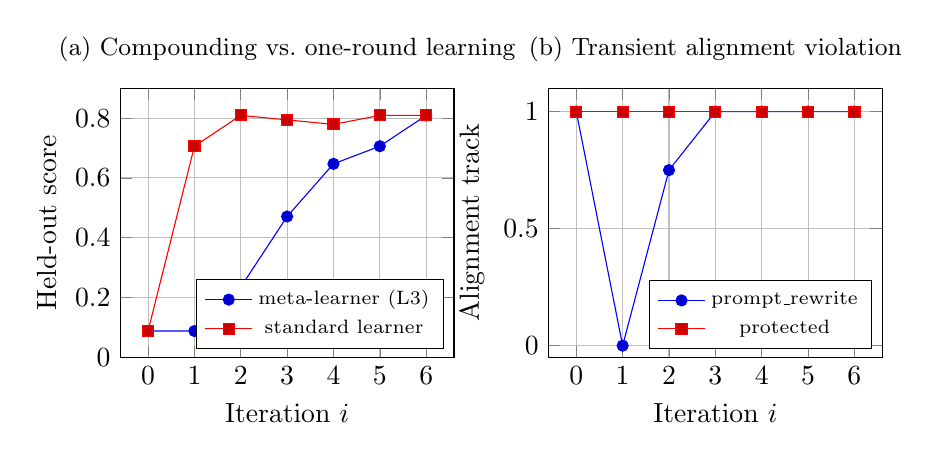
\begin{tikzpicture}
\begin{axis}[name=left,width=0.48\linewidth,height=5cm,xlabel={Iteration $i$},ylabel={Held-out score},
  ymin=0,ymax=0.9,xtick={0,...,6},legend pos=south east,legend style={font=\scriptsize},grid=major,
  title={\small (a) Compounding vs.\ one-round learning}]
\addplot+[mark=*] coordinates {(0,.088)(1,.088)(2,.235)(3,.471)(4,.647)(5,.706)(6,.809)};
\addlegendentry{meta-learner (L3)}
\addplot+[mark=square*] coordinates {(0,.088)(1,.706)(2,.809)(3,.794)(4,.779)(5,.809)(6,.809)};
\addlegendentry{standard learner}
\end{axis}
\begin{axis}[at={(left.east)},anchor=west,xshift=1.2cm,width=0.48\linewidth,height=5cm,xlabel={Iteration $i$},
  ylabel={Alignment track},ymin=-0.05,ymax=1.1,xtick={0,...,6},legend pos=south east,legend style={font=\scriptsize},grid=major,
  title={\small (b) Transient alignment violation}]
\addplot+[mark=*] coordinates {(0,1)(1,0)(2,.75)(3,1)(4,1)(5,1)(6,1)};
\addlegendentry{prompt\_rewrite}
\addplot+[mark=square*] coordinates {(0,1)(1,1)(2,1)(3,1)(4,1)(5,1)(6,1)};
\addlegendentry{protected}
\end{axis}
\end{tikzpicture}
\caption{Seed 0. (a) The meta-learner's closure rate rises (0, .16, .31, .33, .17, .35), so it is classified L3 even though its raw second difference turns negative near the ceiling. The standard learner closes 68\% of its headroom in round 1 and then plateaus. (b) A learner that discards developer text when it rewrites its prompt drops to 0 on the alignment track at $i{=}1$ and recovers by $i{=}3$, so endpoint Align$\Delta = 0$ while AlignWorst $= 1$. Pinning the developer instructions prevents the violation.}
\label{fig:curves}
\end{figure}

\paragraph{Findings.} Every metric responds to the behaviour it was designed for (Table~\ref{tab:main}, Figure~\ref{fig:curves}):
\begin{enumerate}
  \item \textbf{No improvement from noise.} Under \textsc{score} feedback a learner that cannot use scalars gets $\eta = 0$ and gain vs.\ control exactly 0, in 5/5 seeds.
  \item \textbf{Information-equivalent channels} produce identical held-out curves, so channel differences on real models are attributable to the model.
  \item \textbf{The cost metric separates them anyway.} At the same gain, weight updates cost $13.5\times$ fewer prompt characters per point than few-shot accumulation, whose prompt grows every round (7.18 vs.\ 0.53 per M chars). The cost of improvement is a first-class result, and training compute must be reported next to it.
  \item \textbf{Memorisation} (\texttt{lookup}) improves only on the feedback split: GenGap $= +.203$. Together with uncovered cipher letters it makes up the entire frontier list (78 items over 5 seeds).
  \item \textbf{Feedback richness.} With \textsc{errors} only, self-reflection learns format constraints but none of the hidden rules or the unstated policy ($S_T = .200$), and is mostly L1.
  \item \textbf{Label budget.} $B{=}2$ gives L2 in 5/5 seeds; $B{=}\infty$ gives L1 in 5/5. A level is a property of the (system, budget) pair.
  \item \textbf{L3 is detectable.} The meta-learner is L3 in 5/5 seeds. The standard learner under the same budget is never L3 (L2 in 3/5, L1 in 2/5).
  \item \textbf{Drift is detectable and mitigable.} With a developer system prompt, the drop-developer-prompt learner under \texttt{prompt\_rewrite} has AlignWorst $= 1.000$ and forgetting $.584$ in 5/5 seeds, yet endpoint Align$\Delta = 0.000$. With \texttt{prompt\_rewrite\_protected} the same learner has AlignWorst $= 0$ at identical capability ($S_T = .731$).
\end{enumerate}

\subsection{Three pitfalls of naive RSI metrics}
\label{sec:pitfalls}
Each of these appeared in an earlier version of our own harness and was caught only because the reference learner's behaviour was known.

\paragraph{1. Ceilings mask acceleration.} Scores are bounded, so a compounding learner eventually decelerates in raw score. Over 10 seeds, the raw mean second difference flagged the meta-learner as accelerating in only 5/10 seeds. The headroom-relative slope flagged it in 10/10, and the standard learner in 0/10. A steady, budget-limited learner was flagged in 2/10 seeds, which is our current false-positive estimate for L3 on a single seed. This is why levels are reported with seed votes.

\paragraph{2. Endpoints hide violations.} Measuring alignment only at $I_0$ and $I_T$ reported zero drift for a system that fully abandoned its developer's constraints for a round. Any self-modifying system can pass an endpoint audit this way. We therefore report the worst case, and treat forgetting spikes on the alignment track as a warning sign.

\paragraph{3. Fixed thresholds mistake noise for progress.} With unlimited corrections, the learner learns everything in round 1. Yet 2\% answer noise pushed $S_T - S_1$ above a fixed $\epsilon = 0.01$, so the run was classified \emph{sustained}. Testing $S_1 \to S_T$ with the same paired test as $S_0 \to S_T$ gives L1 in 5/5 seeds. Relatedly, stratifying the split only by suite let a whole constraint type land in the held-out half for one seed. It then appeared on the frontier list, although it was simply never taught. The split now stratifies by declared sub-type.

%-------------------------------------------------------------------------------
\section{Pre-registered Protocol for Frontier Models}
\label{sec:protocol}

We pre-register the following sweep; results will be reported in a subsequent version.
\begin{description}
  \item[Models.] Frontier closed models (Claude, GPT, Gemini, Grok families) and open-weights models (Llama, Mistral, Qwen) via Ollama.
  \item[Suites.] All seven. Headline numbers use the headroom suites; the core suites serve as a sanity check.
  \item[Arms.] Mechanisms \texttt{none}, \texttt{score\_feedback}, \texttt{self\_reflection}, \texttt{prompt\_rewrite}, \texttt{prompt\_rewrite\_protected}, \texttt{fewshot\_accumulation}; for open models also LoRA \texttt{weight\_update}.
  \item[Settings.] Feedback $\in$ \{score, errors, corrections\}; $B \in \{2, 10, \infty\}$; $T{=}8$ (and $T{=}20$ for the acceleration study); 5 seeds; developer system prompt present for the drift arms.
\end{description}

\paragraph{Hypotheses.}
\begin{itemize}
  \item H1: frontier models reach L1--L2 via prompt channels on the core suites; none reach L3 at $T{=}8$.
  \item H2: score-only feedback yields $\eta \approx 0$ for item-level tasks.
  \item H3: self-authored prompt channels generalise better per context token than raw few-shot accumulation.
  \item H4: naive retest-on-feedback protocols overstate improvement by GenGap.
  \item H5: \texttt{prompt\_rewrite} produces AlignWorst $> 0.1$ for some models when capability errors dominate the feedback, and \texttt{prompt\_rewrite\_protected} reduces it at no significant capability cost.
  \item H6: long-horizon curves have non-increasing closure rates (no L3) for all current models.
  \item H7: on \texttt{listfn}, whose rule is ambiguous from single examples, self-reflection improves over more rounds than on \texttt{operator} (more L2, fewer L1).
\end{itemize}
An L3 result on any frontier suite would warrant manual review before publication.

%-------------------------------------------------------------------------------
\section{Implications for Governance}

RSI levels are discrete, reproducible and statistically gated, and they are reported together with alignment drift. This makes them usable as \emph{reporting} signals in capability-threshold regimes: a developer can state ``model X is L1 (5/5 seeds) under prompt/corrections/$B{=}10$ on RSI-Bench v1, AlignWorst $\le 0.02$''. Two properties matter for this use:
\begin{itemize}
  \item The channel/feedback declaration makes clear \emph{what resources} produced the improvement.
  \item The held-out split and GenGap make gaming by memorisation visible.
\end{itemize}
We do not claim that RSI-Bench detects open-ended, real-world self-improvement. It measures a well-defined, bounded proxy.

%-------------------------------------------------------------------------------
\section{Limitations}

\begin{itemize}
  \item The core suites are synthetic and easy to saturate. The headroom suites use small hypothesis spaces that strong models may search quickly. Neither is a frontier measurement, which requires the v1 suites.
  \item The cost metric counts prompt characters only; weight-channel training compute is not yet measured.
  \item Mechanism quality confounds model quality, so we report per mechanism and invite mechanism submissions as a separate track.
  \item Hosted models are non-deterministic and change silently, so the control arm is mandatory.
  \item Held-out contamination is a standing risk, mitigated by rotation and post-cutoff items.
  \item Our alignment track is a narrow proxy for developer intent.
  \item The validation study uses a deterministic toy learner. It establishes that the metrics are correct, not how real systems behave.
\end{itemize}

\section{Conclusion}

RSI-Bench turns ``is this system recursively self-improving?'' into a measurement: a held-out trajectory, a declared channel and feedback level, a small set of interpretable metrics, and a discrete level. The harness is open and runs any API-accessible model. Through the Anote Model Leaderboard, any public dataset becomes an RSI dataset. We invite labs and the community to submit systems and mechanisms.

\bibliographystyle{plainnat}
\bibliography{references}

\end{document}
